\documentclass[a4paper, 12pt]{article}
\usepackage[top=2cm, bottom=2cm, left=2.2cm, right=2.2cm]{geometry}
\usepackage[utf8]{inputenc}
\usepackage{amsmath, amsfonts, amssymb}
\usepackage{amsthm}
\usepackage{indentfirst}
\usepackage{graphicx}
\usepackage{gensymb}
\usepackage{float}
\title{Universidade de São Paulo \\ EESC}
\author{SEM0530 - Problemas de Engenharia Mecatrônica II \\ 
Prof. Marcelo Areias Trindade \\ \\ Prática 1 - Zeros de funções
\\ \\ Aluno: Marcus Vinícius Costa Reis (12549384)}
\date{18/05/2022}

\begin{document}
	\maketitle \newpage \tableofcontents \newpage
	
	\section{Problema}
	
	\begin{itemize}
		\item Determinar o deslocamento estático (devido ao peso) de uma suspensão automotiva (oblíqua),
		i.e. encontrar $u$ para o qual o equilíbrio estático é alcançado.
		\item Deseja-se também calcular e visualizar graficamente como a rigidez efetiva ($k_{ef}$) varia com $u$ e o
		valor de rigidez efetiva na proximidade da(s) configuração(ões) de equilíbrio estático.	
	\end{itemize}
	
	\textbf{Dados:}
	
	\begin{itemize}
		\item $d=0.2\,m$, $L=0.5\,m$, $k=10\,kN/m$, $g=9.81\,m/s^2$
		\item $M=(180+N)\,kg$, onde $N$ é formado pelos dois últimos algarismos do N° USP.
		
		Neste caso, $84$. Logo, $M=264\,kg$.		
	\end{itemize}
	
	\subsection{Formulações}
	
	\subsubsection{Parte 1}
	
	Em primeira análise, é válido destacar que em decorrência da aplicação da carga $W$ sobre a estrutura, ocorre um 
	deslocamento $u$ vertical para baixo, de modo que a componente vertical da força restauradora proveniente das molas, 
	responsável por balancear a ação da carga, dependa de $u$.
	
	A Figura 1 mostra uma situação geral, na qual a estrutura se encontra deslocada de $u$ a partir do ponto superior 
	inicial. As molas encontram-se comprimidas de um $\Delta L=L-L_f$, onde $L_f$ é o comprimento das mesmas na situação 
	em questão. Pela geometria, segue que $$L_f^2=(h-u)^2+d^2=h^2+d^2+u^2-2hu=L^2+u(u-2h)$$
	$$\Longrightarrow L_f=\sqrt{L^2+u(u-2h)}\,\,\,(1)$$
	
	A Figura 2 mostra o diagrama de equilíbrio estático para o ponto material superior. Adotando-se o eixo $y$ positivo 
	vertical para cima, tem-se para o somatório de forças na vertical:
	$$\sum F_y=0\Longrightarrow 2f_m\sin \theta -W=0$$ $$\Longleftrightarrow 2f_m\sin \theta =W\,\,\,(2)$$
	
	Evidencia-se, também, que $\sin \theta$ é função de $u$, e segue a relação:
	$$\sin \theta = \frac{h-u}{L_f}\Longleftrightarrow \sin \theta \stackrel{(1)}{=} 
	\frac{h-u}{\sqrt{L^2+u(u-2h)}}\,\,\,(3)$$
	
	Em seguida, pela Lei de Hooke, tem-se que a força elástica $f_m$ das molas segue a equação:
	$$f_m=-k(L_f-L)=k(L-L_f)$$ $$\Longrightarrow f_m=k\left[L-\sqrt{L^2+u(u-2h)}\right]\,\,\,(4)$$
	
	Por meio das equações 1, 2, 3 e 4, chega-se a uma equação envolvendo $u$:
	$$\frac{2k\left[L-\sqrt{L^2+u(u-2h)}\right](h-u)}{\sqrt{L^2+u(u-2h)}}=W\,\,\,(5)$$
	
	\newpage
	
	Expandindo, tem-se: $$\frac{2kL(h-u)}{\sqrt{L^2+u(u-2h)}}-2k(h-u)=W \Longleftrightarrow 
	\frac{2kL(h-u)}{\sqrt{L^2+u(u-2h)}}=W+2k(h-u)$$
	
	Quadrando ambos os membros da equação: $$\frac{4k^2L^2(h-u)^2}{L^2+u(u-2h)}=W^2+4Wk(h-u)+4k^2(h-u)^2$$
	
	Tendo em vista a forma complicada da expressão anterior e objetivando a possível obtenção de um polinômio, 
	realizou-se a mudança de variável $v(u)=h-u$. Assim:
	
	$$\frac{4k^2L^2v^2}{L^2-(h^2-v^2)}=W^2+4Wkv+4k^2v^2$$ 
	$$\Longleftrightarrow 4k^2L^2v^2=(W^2+4Wkv+4k^2v^2)[L^2-(h^2-v^2)]$$
	
	Expandindo: $$4k^2L^2v^2=W^2L^2+4WkL^2v+4k^2L^2v^2-W^2(h^2-v^2)-4Wkv(h^2-v^2)-4k^2v^2(h^2-u^2)$$
	
	Organizando: $$(4k^2)v^4+(4Wk)v^3+(W^2-4k^2h^2)v^2+[4Wk(l^2-h^2)]v+W^2(l^2-h^2)=0$$
	$$\Longleftrightarrow g(v)=(4k^2)v^4+(4Wk)v^3+(W^2-4k^2h^2)v^2+[4Wk(l^2-h^2)]v+W^2(l^2-h^2)$$
	
	Desse modo, chegou-se a um polinômio de grau $4$ em $v$. Após a determinação de suas raízes, pode-se simplesmente 
	retomar a mudança de variável e encontrar os respectivos valores para $u$.
	
	\begin{figure}[!htb]
		\centering
		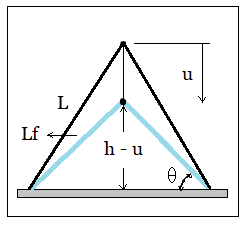
\includegraphics[scale=0.7]{img6.png}
		\caption{Situação geral (sistema deslocado de $u$)}
	\end{figure}
	
	\begin{figure}[!htb]
		\centering
		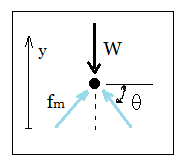
\includegraphics[scale=0.7]{img7.png}
		\caption{Diagrama de forças para o ponto material}
	\end{figure}
	
	\subsubsection{Parte 2}
	
	Agora, volta-se o foco para a análise da rigidez efetiva ($k_{ef}$) do sistema em questão, bem como sua dependência 
	em relação a $u$.
	
	A ideia baseia-se em encontrar um sistema hipotético equivalente ao original, no qual a carga $W$ seja balanceada 
	por uma força de mola equivalente $f_{m_e}$, que será dada por $$f_{m_e}=k_{ef}u\,,$$ onde $u$ é o deslocamento
	no sistema original.
	
	Sendo assim, $f_{m_e}$ deve ter módulo igual a $2f_m\sin \theta$, a resultante das forças elásticas na vertical 
	para o caso original. Logo: $$f_{m_e}=k_{ef}u \Longrightarrow k_{ef}u=2f_m\sin \theta$$
	$$\Longleftrightarrow k_{ef}\stackrel{(3),(4)}{=}2k\frac{\left[L-\sqrt{L^2+u(u-2h)}\right]}{
	\sqrt{L^2+u(u-2h)}}\left(\frac{h}{u}-1\right)\,\,\,(6)$$ $$ $$
	
	A expressão acima será analisada posteriormente.
	
	\newpage
	
	\subsection{Resultados}
	
	\subsubsection{Parte 1}
	
	A partir do polinômio $g$ de quarto grau em $v$ encontrado antriormente, foi possível colocar seus coeficientes no
	prompt do software Octave e, por meio do método interno \textit{roots()}, encontrar os valores de $v$ para os quais
	$g(v)=0$.
	
	Antes, porém, utilizou-se dos dados numéricos do problema para determinar o polinômio:
	$$g(v)=400v^4+103.59v^3-77.293v^2+4.1437v+0.2683\,\,\,(7)$$
	
	Vale ressaltar que foi utilizado $W=Mg=(264\,kg)(9.81\,m/s^2)=2.5898\,kN$, bem como $h=0.4583\,m$, obtido a partir
	da relação $h=(L^2-d^2)^{1/2}$.
	
	Chegou-se, então, aos seguintes valores para $v$: $$v_1=-0.604\,m\,,\,\,v_2=0.275\,m\,,\,\,v_3=0.108\,m
	\,,\,\,v_4=-0.037\,m$$
	
	De posse da relação de mudança de variável ($v(u)=h-u$), pôde-se isolar $u$ ($u(v)=h-v$) e encontrar, por fim, os 
	possíveis valores para o deslocamento estático do sistema:
	$$u_1=1.0624\,m\,,\,\,u_2=0.1835\,m\,,\,\,u_3=0.3504\,m\,,\,\,u_4=0.4957\,m$$
	
	Sabe-se, no entanto, que o deslocamento está restrito ao intervalo $(0,h)=(0,0.4583)$, do ponto superior ao anteparo.
	Dessa forma, os valores de $u$ para o equilíbrio são apenas $u_2$ e $u_3$. Renomeando-os:
	$$u_I=0.1835\,m\,,\,\,u_{II}=0.3504\,m$$
	
	\subsubsection{Parte 2}
	
	Nesta etapa, serão apenas apresentados os valores de rigidez efetiva associados a $u_I$ e $u_{II}$. O comportamento
	da função $k_{ef}(u)$ será discutido posteriormente.
	
	Antes, porém, vale reescrever a equação 6 utlizando os valores numéricos das constantes:
	$$k_{ef}=\frac{20[0.5-\sqrt{0.25+u(u-0.9165)}](0.4583-u)}{u\sqrt{0.25+u(u-0.9165)}}$$
	
	Assim, chegou-se aos seguintes valores utilizando $u=u_I$ e $u=u_{II}$: 
	$$k_{ef}^{I}=14.115\,kN/m\,,\,\,k_{ef}^{II}=7.3923\,kN/m$$ 
			
	
	\newpage
	
	\subsection{Gráficos}
	
	\subsubsection{Parte 1}
	
	Utilizando-se o Octave, foi possível plotar o gráfico correspondente ao polinômio $g$. 
	
	Escolheu-se um intervalo 
	conveniente no eixo das abcissas para poder abranger as quatro raízes do polinômio. Todavia, o trecho de interesse
	está compreendido apenas no intervalo $(0,0.4583)$, cujos extremos correspondem a $u=h=0.4583$ e $u=0$, respectivamente.
	
	O Gráfico 1 mostra tal empreitada.
	
	\begin{figure}[H]
		\centering
		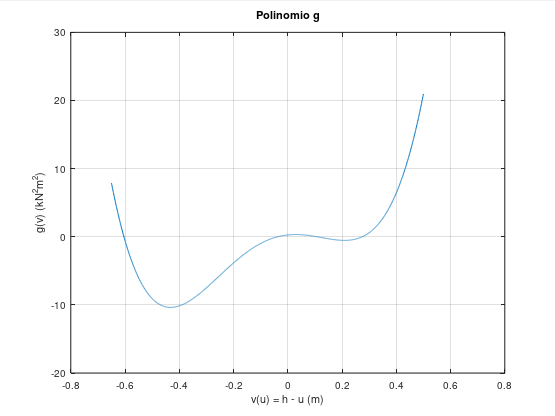
\includegraphics[scale=1]{g1.png}
		\caption{Curva do polinômio g (Gráfico 1)}
	\end{figure}
	
	\subsubsection{Parte 2}
	
	O foco, no entanto, está na análise do gráfico que representa a curva de rigidez efetiva e sua variação com respeito 
	ao deslocamento	estático $u$. O último pôde ser também gerado por meio do Octave, no qual, novamente, escolheu-se uma 
	região de interesse	para destacar.
	
	O resultado de tal ação é mostrado no Gráfico 2.
	
	Faz-se importante, primordialmente, a análise da curva para duas situações, sendo elas: quando o deslocamento $u$ tende
	a ser nulo ($u\rightarrow 0$) e quando $u$ tende a $h$ ($u\rightarrow h$).
	
	Iniciando pela primeira situação, é válido interpretar seu significado no contexto do problema original. O deslocamento
	estático em questão ocorre em decorrência da ação da carga $W$ aplicada, como já citado anteriormente.  Sendo assim, se
	$u$ tende a zero, então o sistema tende a uma situação na qual inexiste aplicação de carga. Portanto, a rigidez efetiva
	será uma equivalência à geometria das molas na situação indeformada. 
	
	Pensando em uma circunstância hipotética na qual
	as molas estivessem ambas na vertical, a rigidez efetiva seria dada por $k_{ef}=2k$. Todavia, como o ângulo entre as 
	molas e o chão é de aprox. $66.43\degree =\sin ^{-1}(h/L)$, espera-se um valor de $k_{ef}$ próximo de $2k=20\,kN/m$.
	
	Observando o Gráfico 2, tem-se que a intuição anterior se mostra correta, tendo em vista que o valor de $k_{ef}$ tende
	a alguma medida entre $16\,kN/m$ e $17\,kN/m$. Vale, ainda, ressaltar, que o ponto exato da curva para o qual $u=0$ não
	é definido, já que, pela eq. 6, estaria-se dividindo a expressão por zero. Trata-se de um ponto de descontinuidade 
	removível.
	
	No que diz respeito à segunda situação (quando $u\rightarrow h$), entende-se que as molas estariam convergindo para uma
	circunstância na qual ambas estariam na horizontal. Dessa maneira, não haveria força restauradora atuando na direção
	vertical, e a rigidez efetiva seria, por conseguinte, nula.	
	
	Pelo gráfico, observa-se que $u=0.4583$ é zero da função, ou seja, $k_{ef}(0.4583)=0$, cofirmando o que foi discutido.
	
	Uma última análise pertinente concerne ao comportamento da curva quando $u\rightarrow -\infty$. Fazendo analogia à 
	situação real, pode-se pensar que o ângulo $\theta$ entre as molas e o anteparo estaria crescendo e tendendo a $\pi /2$,
	de forma que, então, as molas tenderiam a estar dispostas na vertical, e paralelas entre si. Desse modo, depreende-se 
	que $k_{ef}$ seria simplesmente $2k$. De fato, a curva tem uma assíntota horizontal em $k_{ef}=20\,kN/m$.
	
	Por fim, vale ressaltar que a partir do ponto de deslocamento $u=h=0.4583\,m$, a curva não possui mais interpretação
	física, já que teria-se atravessado a linha do anteparo.
	
	\begin{figure}[!htb]
		\centering
		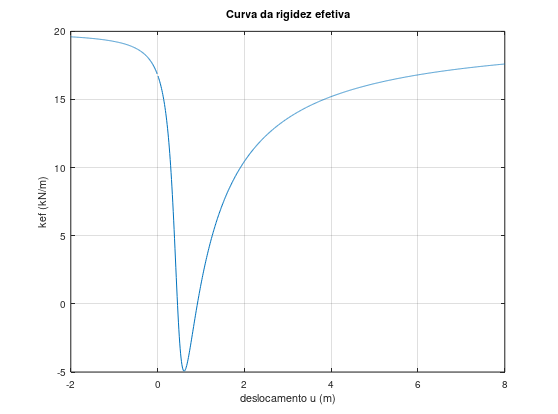
\includegraphics[scale=1]{g2.png}
		\caption{Curva de rigidez efetiva (Gráfico 2)}
	\end{figure}
	
	\subsection{Análise do equilíbrio}
	
	Como foram encontrados dois valores distintos para o deslocamento estático $u$ que satisfazem o equilíbrio da estrutura, 
	faz-se conveniente analisar a establidade do equilíbrio em cada ponto encontrado. 
	
	Para tal, pode-se interpretar o 
	polinômio $g$ como a primeira derivada de uma função primitiva $G$, que não tem relação com o problema no momento. Fato é,
	como os valores de $v$ encontrados são raízes de $g$, faz-se analogia à determinação de máximos e mínimos de funções 
	(nesse caso seria analisada a primitiva $G$) para se utilizar do teste da segunda derivada e concluir a respeito da 
	estabilidade do equilíbrio.
	
	Desse modo, a função segunda derivada de $G$ é a derivada primeira de $g$, de modo que se obtém:
	$$z(v)=g'(v)\stackrel{(7)}{=}1600v^3+310.77v^2-154.586v+4.1437$$	
	
	Utilizando o Octave, calculou-se o valor de $z$ nos pontos $v_2$ e $v_3$ (correspondentes a $u_I$ e $u_{II}$). Obteve-se:
	$$z(v_2)=18.316>0\,,\,\,\,z(v_3)=-6.9075<0$$
	
	Dessa forma, conclui-se que o equilíbrio em $u=u_I$ é \textit{estável}, enquanto em $u=u_{II}$, \textit{instável}.
	
	Uma possível explicação sobre esses resultados pode ser obtida quando se observam os valores de $k_{ef}$ em cada situação.
	Para $u=u_{II}$, o valor da rigidez efetiva é inferior à rigidez de cada mola sozinha. Isso aponta para uma certa 
	instabilidade. Para $u=u_{I}$, esse valor é quase o dobro.
	
	Ademais, se há uma desestabilização em $u=u_{II}$, o sistema tende a retornar para a posição $u=u_{I}$, de equilíbrio
	estável.
	
	\subsection{Scripts}
	
	As figuras que se seguem mostram os scripts em Octave utilizados para os cálculos anteriores, bem como para a geração
	dos gráficos.
	
	\begin{figure}[!htb]
		\centering
		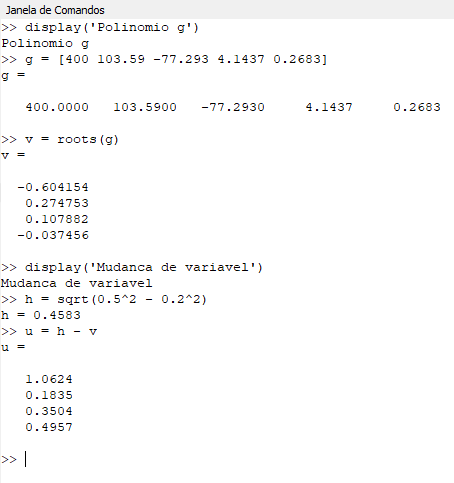
\includegraphics[scale=0.7]{img1.png}
		\caption{Valores de $u$}
	\end{figure}
	
	\begin{figure}[H]
		\centering
		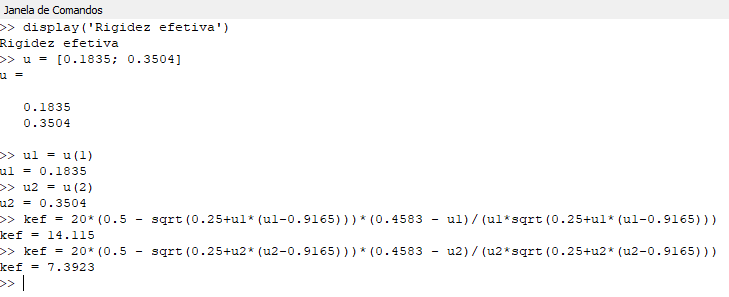
\includegraphics[scale=0.7]{img2.png}
		\caption{Valores de $k_{ef}$}
	\end{figure}
	
	\begin{figure}[H]
		\centering
		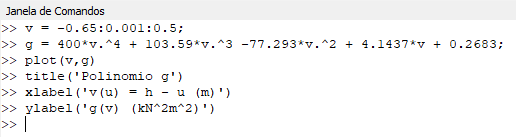
\includegraphics[scale=0.7]{img3.png}
		\caption{Plot do polinômio $g$}
	\end{figure}
	
	\begin{figure}[H]
		\centering
		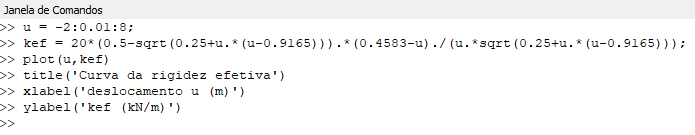
\includegraphics[scale=0.7]{img4.png}
		\caption{Plot da curva de rigidez efetiva}
	\end{figure}
	
	\begin{figure}[H]
		\centering
		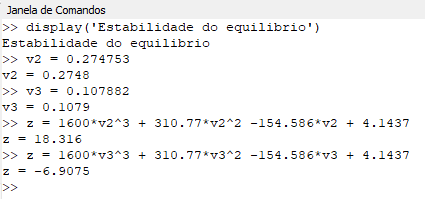
\includegraphics[scale=0.7]{img5.png}
		\caption{Estabilidade do equilíbrio}
	\end{figure}
	
	\newpage
	
	\section{Conclusões}
	
	Em primeira instância, pode-se dizer que foi realizada uma análise minimamente razoável do problema proposto, de forma
	que se fez possível a determinação de duas configurações de equilíbrio estático para a estrutura envolvida, as quais 
	puderam ser caracterizadas com valores de deslocamento e rigidez efetiva.
	
	O trabalho com as formulações e equações envolvidas foi conduzido de maneira que as soluções se mostraram coerentes
	com o problema físico, sobretudo quando se observa o comportamento dos gráficos que foram construídos.
	
	Por fim, pode-se afirmar que o uso do Octave como ferramenta computacional auxiliou grandemente na visualização e
	construção do que foi apresentado anteriormente. 
			
\end{document}






